% Financial Reporting Process Flowchart
% TikZ diagram for Chapter 2

\documentclass[tikz,border=10pt]{standalone}
\usepackage{tikz}
\usetikzlibrary{shapes,arrows,positioning,fit,backgrounds}

\begin{document}

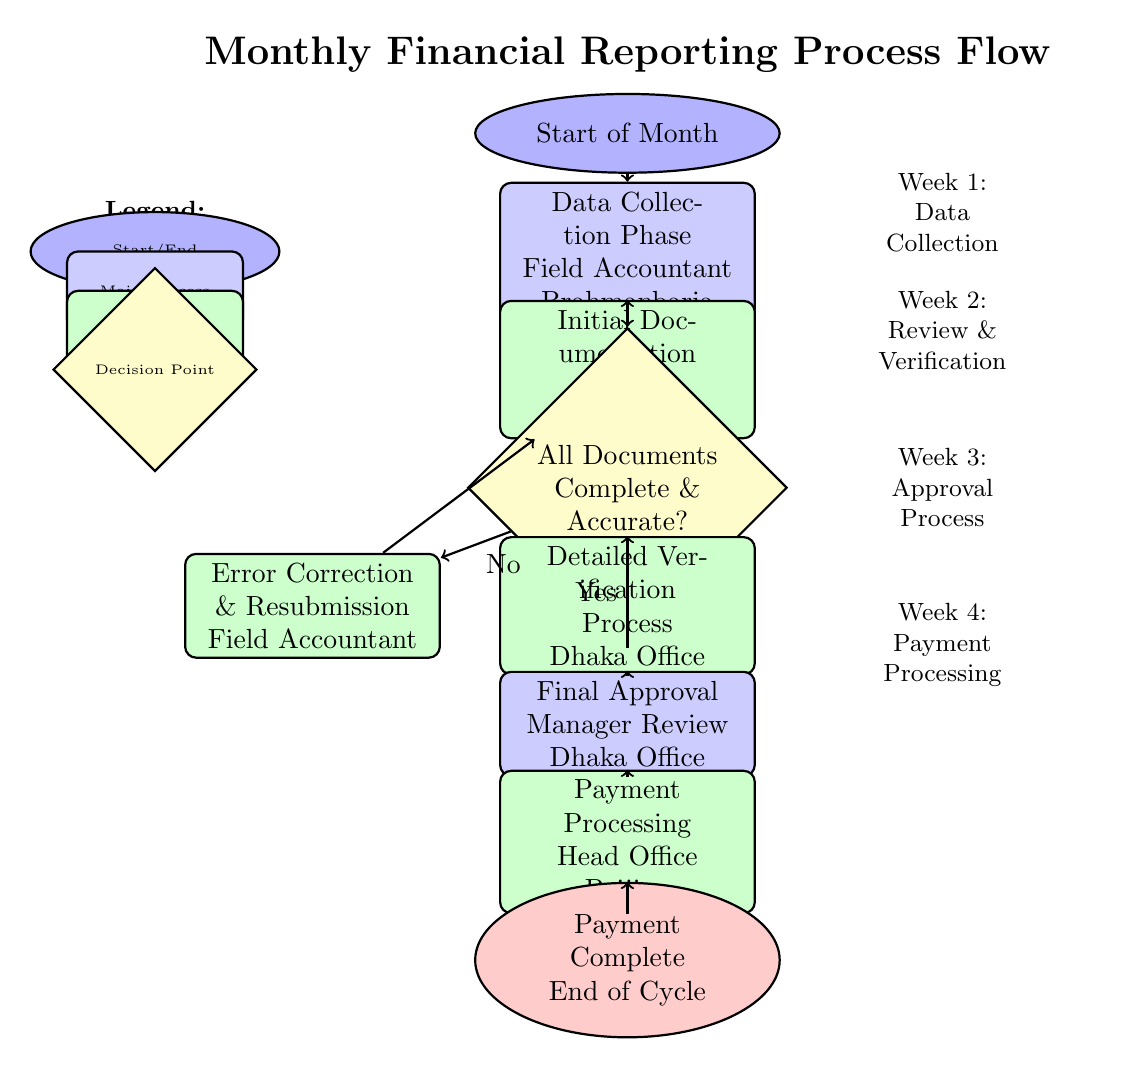
\begin{tikzpicture}[
    node distance=1.5cm,
    auto,
    thick,
    main node/.style={rectangle, draw, fill=blue!20, text width=3cm, text centered, rounded corners, minimum height=1cm},
    decision node/.style={diamond, draw, fill=yellow!20, text width=2.5cm, text centered, minimum height=1cm},
    process node/.style={rectangle, draw, fill=green!20, text width=3cm, text centered, rounded corners, minimum height=1cm},
    start node/.style={ellipse, draw, fill=blue!30, text width=2.5cm, text centered, minimum height=1cm},
    end node/.style={ellipse, draw, fill=red!20, text width=2.5cm, text centered, minimum height=1cm}
]

% Title
\node[text width=12cm, text centered, font=\Large\bfseries] (title) at (0,8) {Monthly Financial Reporting Process Flow};

% Start
\node[start node] (start) at (0,7) {Start of Month};

% Data Collection
\node[main node] (data_collection) at (0,5.5) {Data Collection Phase\\Field Accountant\\Brahmanbaria};

% Initial Review
\node[process node] (initial_review) at (0,4) {Initial Documentation\\Review\\Dhaka Office};

% Verification Decision
\node[decision node] (verification) at (0,2.5) {All Documents\\Complete \&\\Accurate?};

% Error Correction
\node[process node] (error_correction) at (-4,1) {Error Correction\\\& Resubmission\\Field Accountant};

% Detailed Verification
\node[process node] (detailed_verification) at (0,1) {Detailed Verification\\Process\\Dhaka Office};

% Final Approval
\node[main node] (final_approval) at (0,-0.5) {Final Approval\\Manager Review\\Dhaka Office};

% Payment Processing
\node[process node] (payment_processing) at (0,-2) {Payment Processing\\Head Office\\Beijing};

% End
\node[end node] (end) at (0,-3.5) {Payment Complete\\End of Cycle};

% Arrows
\draw[->] (start) -- (data_collection);
\draw[->] (data_collection) -- (initial_review);
\draw[->] (initial_review) -- (verification);
\draw[->] (verification) -- node {No} (error_correction);
\draw[->] (verification) -- node {Yes} (detailed_verification);
\draw[->] (error_correction) -- (initial_review);
\draw[->] (detailed_verification) -- (final_approval);
\draw[->] (final_approval) -- (payment_processing);
\draw[->] (payment_processing) -- (end);

% Timeline annotations
\node[text width=2cm, text centered, font=\small] (timeline1) at (4,6) {Week 1:\\Data Collection};
\node[text width=2cm, text centered, font=\small] (timeline2) at (4,4.5) {Week 2:\\Review \&\\Verification};
\node[text width=2cm, text centered, font=\small] (timeline3) at (4,2.5) {Week 3:\\Approval\\Process};
\node[text width=2cm, text centered, font=\small] (timeline4) at (4,0.5) {Week 4:\\Payment\\Processing};

% Legend
\node[text width=3cm, text centered, font=\small\bfseries] (legend_title) at (-6,6) {Legend:};
\node[start node, text width=2cm, font=\tiny] (legend_start) at (-6,5.5) {Start/End};
\node[main node, text width=2cm, font=\tiny] (legend_main) at (-6,5) {Main Process};
\node[process node, text width=2cm, font=\tiny] (legend_process) at (-6,4.5) {Sub Process};
\node[decision node, text width=2cm, font=\tiny] (legend_decision) at (-6,4) {Decision Point};

\end{tikzpicture}

\end{document}
